%\usepackage{xspace}

\newcommand{\bits}{\{0,1\}}
\newcommand{\bfu}{\mathbf{u}}
\newcommand{\bfv}{\mathbf{v}}
\newcommand{\bfp}{\mathbf{p}}
\newcommand{\bfz}{\mathbf{z}}
\newcommand{\bfx}{\mathbf{x}}
\newcommand{\bfy}{\mathbf{y}}

\newcommand{\calR}{\mathcal{R}}

\newcommand{\CNextMsg}{\ensuremath{{\sf C Next Msg}}}
\newcommand{\SNextMsg}{\ensuremath{{\sf S Next Msg}}}
\newcommand{\CNext}{\ensuremath{{\sf C Next}}}
\newcommand{\SNext}{\ensuremath{{\sf S Next}}}
\newcommand{\Cstp}{\ensuremath{{\sf Cst'}}}
\newcommand{\Cst}{\ensuremath{{\sf Cst}}}
\newcommand{\msg}{\ensuremath{{\sf msg}}}
\newcommand{\msgp}{\ensuremath{{\sf msg'}}}
\newcommand{\Coutput}{\ensuremath{{\sf Reconstr}}}
\newcommand{\ans}{\ensuremath{{\sf ans}}}
\newcommand{\Ccoins}{\ensuremath{{\sf Ccoins}}}
\newcommand{\Scoins}{\ensuremath{{\sf Scoins}}}
\newcommand{\Expt}{\ensuremath{{\sf Expt}}}
\newcommand{\coin}{\ensuremath{{\sf coin}}}
\newcommand{\View}{\ensuremath{{\sf View}}}
\newcommand{\PPT}{PPT }
\newcommand{\Out}{\ensuremath{{\sf Out}}}
\newcommand{\OWF}{\ensuremath{{\sf OWF}}}
\newcommand{\OT}{\ensuremath{{\sf OT}}}
\newcommand{\PIR}{\ensuremath{{\sf PIR}}}
\newcommand{\Server}{\ensuremath{{\sf Server}}}
\newcommand{\Client}{\ensuremath{{\sf Client}}}
\newcommand{\Alice}{\ensuremath{{\sf Alice}}}
\newcommand{\Bob}{\ensuremath{{\sf Bob}}}
\newcommand{\get}{\ensuremath{\leftarrow}}
\newcommand{\E}{\ensuremath{{\bf E}}}
\newcommand{\out}{\ensuremath{{\sf out}}}
\newcommand{\addr}{\vec{\mbox{addr}}}
\newcommand{\action}{\vec{\mbox{action}}}
\newcommand{\op}{\vec{\mbox{op}}}
\newcommand{\mread}{\mbox{read}}
\newcommand{\mwrite}{\mbox{write}}

\newcommand{\red}[1]{{}\color{red}#1}

\tikzset{every tree node/.style={minimum width=2em,draw},
         blank/.style={draw=none},
         edge from parent/.style=
         {draw,edge from parent path={(\tikzparentnode) -- (\tikzchildnode)}},
         level distance=1.5cm}

In this lecture, we will prove that any Oblivious RAM (ORAM)
scheme must suffer from logarithmic overhead. 
We will show two proofs.  The first
proof was 
described in Goldreich and Ostrovsky's original paper on 
ORAM~\cite{goldreich96software}. 
Their lower bound has two restrictions: 
1) it works only for {\it statistically} secure ORAMs and 
2) 
it assumes that the ORAM is in the {\it balls-and-bins}
model, i.e., the scheme does not perform
any encoding on the payload strings stored in memory.
Many years later, in 2018, the 
work of Larsen and Nielsen~\cite{larsen18lowerbound}
proved a new lower bound removing both of these restrictions. 
Interestingly, their proof uses techniques
from the data structure lower bound literature.
We will also 
cover Larsen and Nielsen's lower bound in today's lecture.




\section{Goldreich and Ostrovsky's Lower Bound}

\begin{theorem}[Goldreich-Ostrovsky ORAM lower bound]
Consider any perfectly secure ORAM scheme in the balls-and-bins model
such that the memory is  
initialized with $n$ words, and the client has $m$ space. 
Then, any 
logical request sequence of length $t$ 
must incur $\max(n, \Omega(t \log_m n))$ total cost. 
Further, the lower bound works even for read-only 
requests. 
\end{theorem}
\begin{proof}
Consider the following game. 
Initially, there are $n$ balls, and ball $i$ is stored in cell $i$
of the memory.
There is a sequence of $t$ logical requests, to read
the balls indexed $i_1, \ldots, i_t$ respectively.
A player 
can hold up to $m$ balls in her hand, and initially, her hand is empty.
In every time step indexed $1, 2, \ldots, q$, she 
can visit a memory cell of her choice and 
take one of the following hidden actions: 
\begin{enumerate}[itemsep=1pt]
\item 
Take a ball from the memory cell and put it in her hand;
\item 
Place a ball from her hand to the memory cell (if it is currently empty);
\item 
Do nothing.
\end{enumerate}
The player's action sequence 
can satisfy the request sequence, iff there is  
a subsequence 
$1\leq j_1 \leq j_2 \leq \ldots \leq j_t \leq q$, such
that for all $k \in [t]$, 
the ball indexed $i_k$ is in the player's hands
at the end of 
time step $j_k$. 

Suppose that an adversary can observe which memory cell
the player visits in every time step,  
but cannot observe which hidden action the player takes. 
Similarly, the adversary cannot observe which balls are 
stored in the memory cells or the player's hands.
Now, the player's job is to satisfy the logical request
sequence $i_1, \ldots, i_t$ without revealing any information 
about the logical request sequence.
We assume that the adversary knows the parameters $n, t, m$.

First, it is easy to see that $q \geq m$. 
To see this, consider a logical request sequence of length $1$.
To satisfy the request, 
if there is some memory cell the player does not visit, it directly
reveals
that the request is not for that index.
In the remainder of the proof, we focus on proving
$q \geq \Omega(t \log_m n)$.

Consider a fixed sequence of memory cells visited 
$(v_1, \ldots, v_q)$ 
that happens with non-zero probability 
when the logical request sequence is $(1, 1, \ldots, 1)$.
%Henceforth we call 
%$(v_1, \ldots, v_q)$ 
%the {\it physical access} sequence.
Because of the privacy requirement, 
$(v_1, \ldots, v_q)$ 
must be able to satisfy any logical request
sequence of length $t$, and the total number
of logical request sequences of length $t$ is $n^t$.

Now, how many logical request sequences
can $(v_1, \ldots, v_q)$ 
satisfy? 
When we fix %the sequence of memory cells visited
the physical access sequence 
$(v_1, \ldots, v_q)$, 
in each of the 
$q$ time steps, the player can choose 
one of at most $m+2$ hidden actions. 
Specifically, if the player chooses to place a ball,
the ball can be 
one of the (up to) $m$ balls in her hand. 
Therefore, fixing $(v_1, \ldots, v_q)$, there are 
$(m+2)^q$ possible 
action sequences.
Further, when we fix the sequence of memory cells
visited $(v_1, \ldots, v_q)$
as well as the sequence of hidden actions, 
it 
satisfy at most ${q \choose t} \cdot m^t$
logical requests, where $q \choose t$ is the number
of ways to choose $t$ out of the $q$ time steps,
and for each of the $t$ chosen time steps, the player can choose
one out of up to $m$ balls in her hand to satisfy the next request.

Summarizing the above, we have
that 
\[
{q \choose t} \cdot (m+2)^q \geq n^t
\]
Using the fact that ${q \choose t} \leq \left(\frac{eq}{t}\right)^t$, we have
\[
\left(\frac{eq}{t}\right)^t\cdot (m+2)^q \geq n^t
\]
Therefore,
\[
q \log(m+2) \geq t (\log n  -  \log (eq/t))
\]
If $q/t > \sqrt{n}$, then $q > t \log n$ trivially follows.
Therefore, we may assume that $q/t > \sqrt{n}$.  
In this case, 
we have that 
$q \geq \Omega(t\log n/\log(m+2))$ which gives the desired bound. 
\end{proof}

Note that the counting-based argument in the above proof
implicitly assumes that the 
scheme is perfectly secure.
Also, the game  
setup
where the player can only grab and place
balls means that this proof works only 
for ORAM schemes in the balls-and-bins model.



\section{Old Text}


\textbf{Goldreich-Ostrovsky Lower Bound \cite{goldreich96software}} Any ORAM scheme (in the balls-and-bins model) must have at least logarithmic overhead. 

\noindent To prove, let
\begin{itemize}
  \item $m =$ number of balls the client can hold in its hand
  \item $t =$ logical request sequence length
  \item $n =$ memory size
\end{itemize}

\noindent Every step, client can visit some memory location $i$, and
\begin{enumerate}
  \item take no action
  \item take a ball from $i$
  \item place a ball into $i$
\end{enumerate}

\noindent Now given
\begin{itemize}
  \item initial memory with $n$ balls,
  \item requests $r_1\dots r_t$
  \item implementation $(\addr, \action)$ and $q = |\addr|$
\end{itemize}
an observer can only see $\addr$ but not $\action$.

\bigskip
\noindent\emph{Q: Assume perfect security, how many request sequences can $\addr$ realize?}
\begin{enumerate}
  \item For every request, there are $m+2$ possible action (1 from doing nothing, 1 from taking a ball, and $m$ from placing a ball).
  \item At the end of each $(\addr, \action)$, the client can use the $m$ balls it has to express $m$ different results.
  \item Need to realize all $n^t$ possible memory access sequences.
\end{enumerate}
Thus,
$$
\begin{array}{rcl}
  (m+2)^q \cdot m^q \geq n^t & \Rightarrow & q\log m + q\log(m+2) \geq t\log n \\
  & \Rightarrow & q/t \geq \frac{\log n}{2\log (m+2)}
\end{array}
$$

\noindent Restrction of G-O LB:
\begin{enumerate}
  \item Balls and bins assumptions
  \item Only works for statistically secure schemes
\end{enumerate}

\section{Lauren-Nielsen}

\textbf{Lauren-Nielsen Lower Bound \cite{larsen18lowerbound}} Logarithmic LB for ORAM but removing these restrictions.

\noindent Assumptions:
\begin{itemize}
  \item read and write in ``word''
  \item word size $\geq \log N$ (memory size)
\end{itemize}

Assume that there is a binary tree, where each leaf node corresponds to a consecutive (read, write) pair. W.L.o.G, fix 
$$\op = \mread(0), \mwrite(0, 0), \dots, \mread(0), \mwrite(0, 0)$$
Want to show: number of probes into memory must be "high" for $\op$.

\noindent \emph{How the tree helps us count}: suppose $\mbox{op}_j$ probes some mem location, and the last time this location was probed was during $\mbox{op}_i$. Then we charge this probe to the least common ancestor in the tree of $\mbox{op}_i$ and $\mbox{op}_j$.

\begin{tikzpicture}
  \Tree
  [.\red{charge}     
      [.{} 
        [.{\dots} ]
        [.\red{$\mbox{op}_i$} ]
      ]
      [.{}
        [.{\dots} ]
        [.\red{$\mbox{op}_j$} ]
      ]
  ]
\end{tikzpicture}

Assume that the adversary can observe the physical probe locations and the boundary between each $\mbox{op}$. Then it can construct this tree in polynomial time, i.e. how many probes are charged to each node. (\emph{This is where computational security kicks in.})

By ORAM security: $\forall\ \op, \op'$ of same length, the two trees constructed must be computationally indistinguishable from each other.

For every subtree $v$ of size $2m$, let the left half of the leaves denote
$$\mread(0), \mwrite(1, r_1)$$
$$\vdots$$
$$\mread(0), \mwrite(m, r_m)$$
and the right half denote
$$(\mread(1), \mwrite(0, 0))$$
$$\vdots$$
$$(\mread(m), \mwrite(0, 0))$$

Idea: when we count the probes assigned to each node $v$, we can use the worst-case sequence for $v$.

Intuition: imagine balls-and-bins model, number of probes assigned to $v \geq\frac{|\mbox{leaves under } v|}{2}$. Thus, at each level, there will be at least $T/2$ probes. Since there are $\log T$ levels, total number of probes at least $O(T \log T)$.

\textbf{Information Transfer Technique} (Encoding Argument): let coins be the randomness consumed by ORAM.
\begin{itemize}
  \item Encode ($r_1, \dots r_m$, coins)
  \begin{enumerate}
    \item Execute ORAM over prefix $\mread(0), \mwrite(0, 0), \dots$
    \item Execute $\mread(0), \mwrite(1, r_1), \dots, \mread(0), \mwrite(m, r_m)$
    \item Execute $\mread(1), \mwrite(0, 0), \dots, \mread(m), \mwrite(0, 0)$
  \end{enumerate}
  \item Encoding ($C$) = for each memory location probed during 2 and 3, record (location, last value written during 2) and the CPU register at the end of 2
  \item Decode ($C$, coins)
  \begin{enumerate}
    \item Same as 1 in Encode
    \item Reset CPU state to $C$.cpuState for every (loc, val) in $C$, let mem[loc]$\leftarrow$ val
    \item same as 3 in Encode
  \end{enumerate}
  \item Decoder output the outcomes of the read ops in 3
\end{itemize}

